\subsection{Datenvorverarbeitung}
\glqq Da die Zieldaten aus den Datenquellen lediglich extrahiert werden, ist im Rahmen der Datenvorverarbeitung die Qualität des Zieldatenbestands zu untersuchen und – sofern nötig – durch den Einsatz geeigneter Verfahren zu verbessern.\grqq\seFootcite{}{S.9}{Cleve.2014}

Diese essentielle Phase verfolgt das Ziel, die unstrukturierten und zunächst nutzlos scheinenden selektierten Rohdaten, in Daten höherer Qualität umzuwandeln, um diese der passenden \gls{dm}-Methode im geeigneten Format bereitzustellen zu können. Die Struktur und das Format muss perfekt auf die vorliegende Aufgabe passen, ansonsten führt die geringe Qualität der Daten zu schlechten bzw. falschen Resultaten bis hin zu Laufzeitfehlern.\seFootcite{Vgl.}{S.10-11}{Garcia.2015} Es gilt auch hier das alte Prinzip: GIGO – garbage in, garbage out.\seFootcite{Vgl.}{S.197}{Cleve.2014} Die oftmals schlechte Qualität der (Roh-)Daten ist durch \textit{fehlende, ungenaue, inkonsistente bzw. widersprüchliche} Daten zu begründen.\seFootcite{Vgl.}{S.84}{Han.2012}\seFootcite{Vgl.}{S.196}{Cleve.2014} Im Folgenden werden dazu einige Ursachen beispielsweise aufgeführt.

Ungenaue bzw. falsche Daten können schon bei der Erhebung entstehen, wenn ein falsches Datenerhebungsinstrument ausgewählt wurde. Bei Stichproben sollte die Gesamtmenge so präzise wie möglich widerspiegeln, um die Datenakkuratesse nicht zu gefährden.\seFootcite{Vgl.}{S.25}{Fahrmeir.2007} Weiterhin können technische und menschliche Fehler zu ungenauen Daten führen, indem Personen beispielsweise ihre persönlichen Informationen bei einer Befragung absichtlich verschleiern (z.B. Standardwert für Geburtsdatum 1. Januar), wobei man diese Problematik auch als \textit{\glqq disguised missing data\grqq}~bezeichnet.\seFootcite{Vgl.}{S.84}{Han.2012}\seFootcite{Vgl.}{S.24}{Fahrmeir.2007}\seFootcite{Vgl.}{S.196}{Cleve.2014} Neben der falschen subjektiven Einschätzung des Menschen bei der Erhebung, können auch aus technischer Sicht ungenaue Daten ermittelt werden, wie z.B. durch (teils-)defekte Sensoren. Nicht zuletzt können Daten bei einem Transfer verfälscht werden bzw. sogar teilweise verloren gehen.\seFootcite{Vgl.}{S.84}{Han.2012}

Fehlenden Daten lassen sich einerseits durch technische Mängel begründen, andererseits auch durch die Tatsache, dass bestimmte Attribute schlichtweg von Beginn aus bei der Erhebung nicht betrachtet wurden oder durch bestimmte Restriktionen nicht verfügbar sind.\seFootcite{Vgl.}{S.84-85}{Han.2012}

Die aufzeigten Beispiele spiegeln nur einen kleinen Teil möglicher Ursachen wider und sollen die Bedeutsamkeit dieser Phase für den Data Mining Prozess aufzeigen. Die Datenvorbereitung stellt dabei einige mächtige Werkzeuge zur Verfügung, um die Datenqualität deutlich zu verbessern:\seFootcite{Vgl.}{S.11 ff.}{Garcia.2015}\seFootcite{Vgl.}{S.196 ff.}{Cleve.2014}\seFootcite{Vgl.}{S.84 ff.}{Han.2012}

\begin{itemize}
\item \textbf{Data Cleaning}: In diesem Schritt werden die Daten bereinigt, indem beispielsweise \textit{fehlerhafte} oder \textit{störende} Daten korrigiert werden. (siehe \vref{dc})
\item \textbf{Data Integration}: Diese Phase beschäftigt sich mit der fehlerfreien Zusammenführung von Daten, da diese oftmals aus mehreren unterschiedlichen Quellen stammen. (siehe \vref{di})
\item \textbf{Data Reduction}: Um die Algorithmen der Data Mining Methoden nutzen zu können, muss die immense Datenmenge reduziert bzw. komprimiert werden, um lange Laufzeiten zu vermeiden. (siehe \vref{dr})
\end{itemize}

Auf die in \vref{werkzeuge} vereinfacht, dargestellten Werkzeuge und ihre Konzepte, wird im Folgenden näher eingegangen.

\begin{figure}[H]
\centering
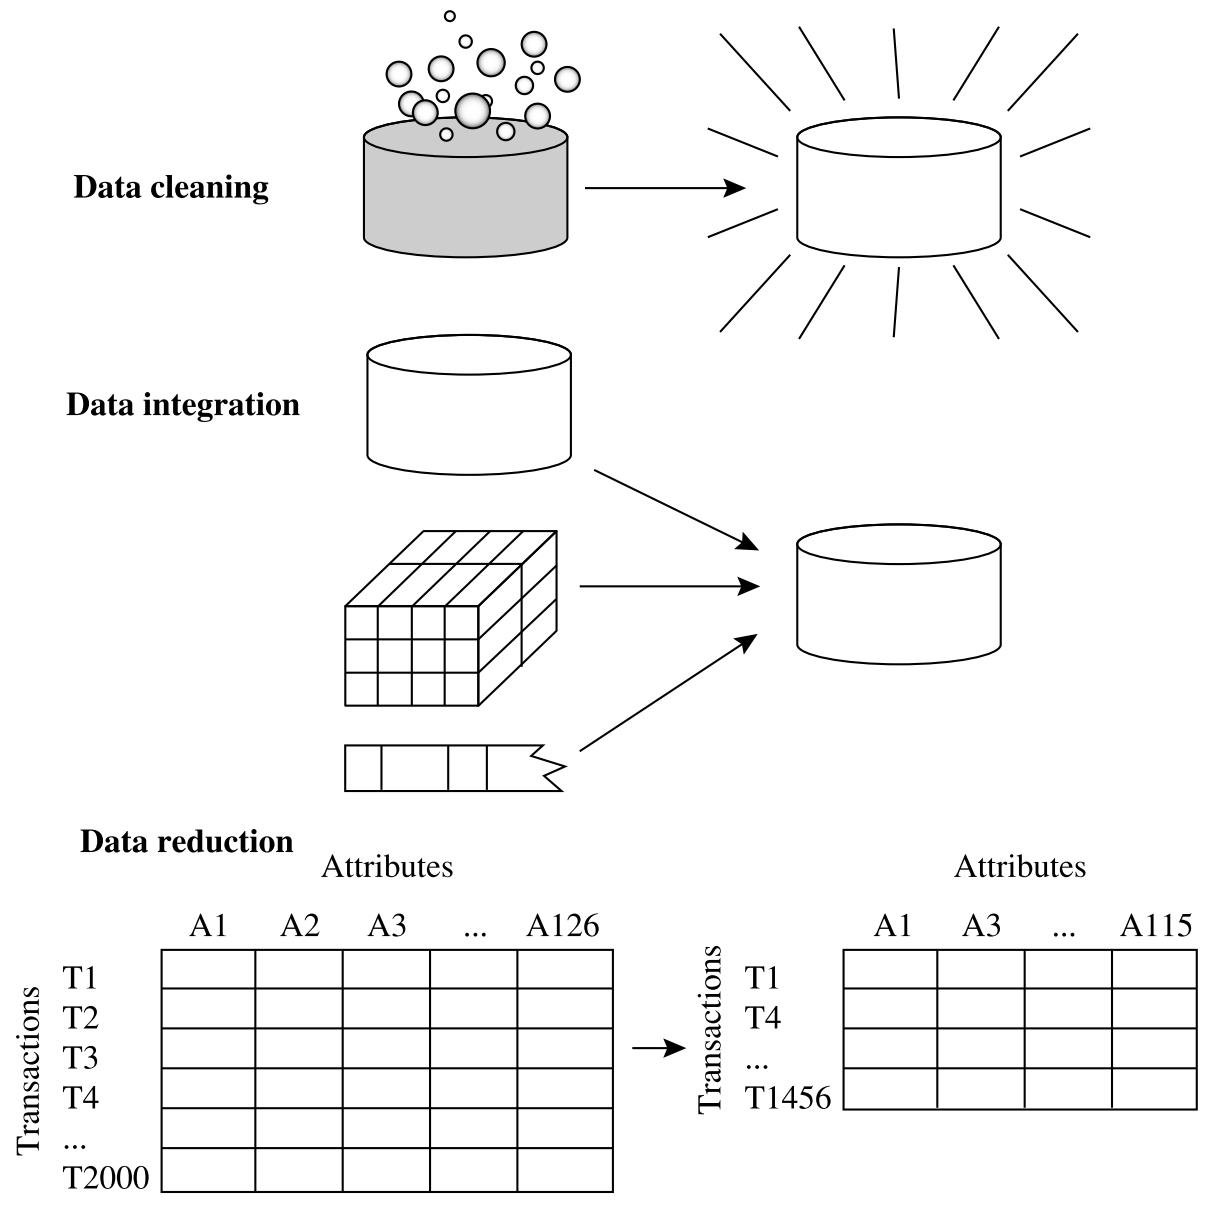
\includegraphics[scale=1.2]{se-wa-jpg/preprocessing}
\caption[Werkzeuge der Datenvorverarbeitung]{Werkzeuge der Datenvorverarbeitung\protect\footnotemark}
\label{werkzeuge}
\end{figure}
\footnotetext{Vgl. Abbildung \textit{Han}, Data Mining: Concepts and techniques, 2012, S.87}


\subsubsection{Data Cleaning}
\label{dc}
In der realen Welt sind Daten häufig \glqq unvollständig, mit Fehlern oder Ausreißer behaftet oder sogar inkonsistent.\grqq\seFootcite{Vgl.}{S.199}{Cleve.2014} Um Fehler oder gar falsche Resultate im Data-Mining-Prozess frühzeitig zu vermeiden, ist es von großer Bedeutung die Datenmenge zu bereinigen. Der Fokus sollte auf der Informationsneutralität liegen, das heißt, es sollen möglichst keine neuen Informationen hinzugefügt werden, die das reale Abbild verzerren oder verfälschen könnten.\seFootcite{Vgl.}{S.199-200}{Cleve.2014} Folgende Problemarten gilt es zu behandeln:\seFootcite{Vgl.}{S.88-90.}{Han.2012}\seFootcite{Vgl.}{S.200-201}{Cleve.2014}

\paragraph{Fehlende Daten} 
Dem Datenanalyst stehen einige Möglichkeiten zur Verfügung, um auf fehlende Daten zu reagieren:

\begin{itemize}
\item \textit{Attribut ignorieren}
\\ Der Datensatz mit dem fehlenden Attribut wird gänzlich ignoriert oder gelöscht. Jedoch können dadurch wichtige Informationen für die Datenanalyse verloren gehen, wodurch dieses Verfahren vor allem bei Datensätzen mit mehreren Lücken angewandt werden sollte.

\item \textit{Manuelles Einfügen}
\\ Besitzt der Datenanalyst das nötige Wissen, kann dieser einzelne Datensätze nachträglich manuell einfügen. Dieser Vorgang entwickelt sich schnell zu einem sehr zeitintensiven und unrealistischen Vorgang, der meistens undurchführbar ist, sobald die Datenmenge wächst. (z.B. 500 Kundendaten per Hand nachtragen)

\item \textit{Globale Konstante}
\\ Den fehlenden Wert durch eine globale Konstante ersetzen, ist sinnvoll, wenn auch ein leeres Feld als Information angesehen wird. Beispiele für Konstanten wären \textsc{unbekannt} oder \textsc{minus unendlich}.

\item \textit{Durchschnittswert}
\\ Handelt sich es bei dem fehlenden Attribut um einen metrischen Wert, so kann der Durchschnittswert aller Einträge als Ersatz verwendet werden. Der Durchschnittswert zeigt sich als äußerst einfache Möglichkeit, wenn die Daten klassifiziert werden können und dadurch Durchschnittswertberechnung nur auf die Datensätze derselben Klasse angewandt wird. Die Methode der \textit{k-Nearest Neighbours} steht zur Verfügung, wenn keine Klassen vorhanden sind, wobei der Durchschnitt, der dem aktuellen Datensatz ähnlichsten Werte benutzt wird.

\item \textit{Wahrscheinlichster oder häufigster Wert}
\\ Durch statistische Methoden kann der wahrscheinlichste Wert für das Attributs ermittelt werden, jedoch sollte dieser Ersatz begründet sein. Bei nicht numerischen Werten kann als weitere Möglichkeit auch der häufigste Wert, als Ersatz für das fehlende Attribut verwendet werden.
\end{itemize}

\paragraph{Verrauschte Daten und Ausreißer}

\begin{itemize}

\item \textit{Klasseneinteilung (bining)}

\item \textit{Regression}

\item \textit{Verbundbildung (clustering)}

\item \textit{Kombinierte Maschine/Mensch-Untersuchung}

\end{itemize}

\paragraph{Falsche und inkonsistente Daten}


\subsubsection{Data Integration}
\label{di}

\subsubsection{Data Reduction}
\label{dr}